\documentclass[12pt]{scrartcl}
\usepackage[utf8]{inputenc}
\usepackage{a4}
\usepackage[none]{hyphenat} %hyphenation
\sloppy
\usepackage{parskip} %no indentation after paragraphs
\usepackage{umlaute}
\usepackage{afterpage} %for using \afterpage{\clearpage} (don't push images to the end of a {\tiny chapter})
\usepackage{makeidx}
\usepackage[numbers]{natbib}
\usepackage{graphicx}
\usepackage{picins} %provides precise control over the placement of inline graphics
\usepackage{setspace}
\usepackage{dsfont} %math symbols
\usepackage{tabularx}
\usepackage{floatflt} %float text around figures and tables

\usepackage{enumitem} %resume counting from previous enumerate block
\usepackage{amsmath,amssymb}
\usepackage[format=default,font=footnotesize,labelfont=bf]{caption}
\usepackage{listings} %for listing source code
\usepackage{color}
\usepackage{algpseudocode} %for listing pseudocode
\usepackage{algorithm} %wrap algpseudocode and enrich with label etc.
\usepackage{float} % for [H] after floats



\makeindex
\frenchspacing
\sloppy

\pagestyle{headings}

\textwidth16cm
\textheight22cm

\topmargin0cm
\oddsidemargin0cm
\evensidemargin0cm


\newcommand{\bildklein}[3]{  
	\begin{figure}[hp]
	\begin{center}
	\includegraphics[width=0.5\textwidth]{#1}
	\end{center}
	\caption[#2]{#3}
	\end{figure}
}
  	
\newcommand{\bildgross}[3]{  
	\begin{figure}[hp]
	\begin{center}
	\includegraphics[width=0.95\textwidth]{#1}
	\end{center}
	\caption[#2]{#3}
	\end{figure}
}
  

\newcommand{\eqn}[3]{
	\begin{figure}[hp]
	\begin{equation}#1\end{equation}
	\caption[#2]{#3}
	\end{figure}
}

\input{figures/tumlogo}

\begin{document}

\nocite{*} %include uncited references in bibliography
\hoffset=5mm
\thispagestyle{empty}

\begin{center}
	\bigskip \bigskip \bigskip 
	\oTUM{6.0cm} \\
	\vspace*{0.8cm}
	{\huge \bf Technische Universität} \\
	\bigskip
	{\huge \bf München} \\
	\bigskip \bigskip \bigskip
	{\huge \bf Fakultät für Informatik} \\
	\bigskip \bigskip \bigskip
	{\Large \bf Seminararbeit in Informatik} \\
	\bigskip \bigskip \bigskip \bigskip \bigskip
	{\Large Die ersten Mikroprozessoren: ein Rechner, ein Chip} \\        
	\bigskip \bigskip \bigskip \bigskip
	{\Large Michael Kratzer, Michael Kiener} \\    
	\bigskip
	\begin{figure}[ht]
	\centering \includegraphics[width=0.2\linewidth]{figures/infologo.jpg}
	\end{figure}
	\bigskip 
\end{center}

\newpage
\tableofcontents

\newpage
\setlength{\baselineskip}{3ex}

\begin{spacing}{1.15}
	\chapter{Einleitung}
\newpage
Test Einleitung
	\section{Der Intel 4004}

\begin{frame}
	\frametitle{Der Intel 4004}
	\framesubtitle{Agenda}
	\begin{enumerate}
		\item Der Intel 4004
		\begin{itemize}
			\item Geschichte des MCS-4
			\item MCS-4
			\begin{itemize}
				\item Der 4001
				\item Der 4002
				\item Der 4003
				\item Der 4004
			\end{itemize}
			\item Funktionsweise des 4004
			\item Auswirkungen auf die Prozessorentwicklung
		\end{itemize}
	\end{enumerate}
\end{frame}

\subsection{Geschichte des MCS-4}

\begin{frame}
	\frametitle{Geschichte des MCS-4}
	\framesubtitle{1968 - Gründung von Intel}
	\begin{columns}[c]
		    \begin{column}{.5\textwidth}
		    	\begin{itemize}
		    		\item Gegründet von Gordon E. Moore und Robert Noyce
		    		\item Hersteller von Speicherchips auf Halbleiterbasis
		    		\item Problem: Kunden zögerten von magnetischen Speichern zu wechseln
		    	\end{itemize}
		    \end{column}
		    \begin{column}{.5\textwidth}
		    	\begin{figure}
		    	    \includegraphics[width=0.7\linewidth]{images/old_intel_logo.png}
		    	\end{figure}
		    \end{column}
	\end{columns}
\end{frame}

\begin{frame}
	\frametitle{Geschichte des MCS-4}
	\framesubtitle{1969 - Auftrag von Busicom}
	\begin{columns}[c]
		\begin{column}{.5\textwidth}
			\begin{itemize}
				\item Spezialauftrag für Busicoms Rechenmaschine
				\item Erstes Design:
				\begin{itemize}
					\item 7 - 12 Chips mit geschätzt 3000 - 5000 Transistoren und 40 Pins
					\item Schieberegister Speicher
					\item komplexes Makroinstruktionsset
				\end{itemize}
				\item Intel hatte keine Erfahrung mit Design von Logikchips
			\end{itemize}
		\end{column}
		\begin{column}{.5\textwidth}
			\begin{figure}[ht]
				 \includegraphics[width=0.8\linewidth]{images/unicom_141P.jpg}
				\caption{Busicom Unicom 141P }
			\end{figure}
		\end{column}
	\end{columns}
\end{frame}

\begin{frame}
	\frametitle{Geschichte des MCS-4}
	\framesubtitle{Neues Design von Intel}
	\begin{columns}[c]
		\begin{column}{.5\textwidth}
			\begin{itemize}
				\item Reduzierung der Komplexität mit Hilfe von größerem Speicher
				\item Mikroinstruktionen
				\item 4-bit Binary Coded Decimal Arithmetik
				\item 3 Chip Design bestehend aus CPU, RAM und ROM
				\item 1900 Transistoren pro Chip
				\item Vergleich zweites Busicom Design: 12 Chips mit 2000 Transistoren und 40 Pins
			\end{itemize}
		\end{column}
		\begin{column}{.5\textwidth}
			\begin{table}[h]
				\begin{tabular}{cc}
					\includegraphics[width=0.35\linewidth]{images/hoff.jpeg}
					%Marcian Edward "Ted" Hoff, Jr.
					& 	
					\includegraphics[width=0.35\linewidth]{images/mazor.jpg}
					%Stanley "Stan" Mazor
					\\
					\includegraphics[width=0.4\linewidth]{images/shima.jpeg}
					% Masatoshi Shima
					& 		\includegraphics[width=0.35\linewidth]{images/faggin.jpg}
					% Federico Faggin
				\end{tabular}
			\end{table}
		\end{column}
	\end{columns}
\end{frame}

\begin{frame}
	\frametitle{Geschichte des MCS-4}
	\framesubtitle{1970 - Entscheidung und Produktion}
	\begin{columns}
		\begin{column}{.5\textwidth}	
				\begin{itemize}
					\item Busicom entscheidet sich Intels Designvorschlag anzunehmen
					\item Intel stellt Federico Faggin als Logik- und Chipdesigner ein
					\item Masatoshi Shima arbeitet an den ersten Programmen für den neuen Prozessor
					\item erster Prototyp nach 9 Monaten fertig
				\end{itemize}
		\end{column}
		\begin{column}{.5\textwidth}
			\begin{figure}[ht]
				\includegraphics[width=1\linewidth]{images/intel_chips.jpg}
				\caption{Intel MCS-4}
			\end{figure}
		\end{column}
	\end{columns}
\end{frame}

\subsection{MCS-4}

\subsubsection{Der 4001}
\begin{frame}
	\frametitle{Der 4001}
	\framesubtitle{Programmierbarer ROM}
	\begin{columns}
		\begin{column}{.5\textwidth}	
			\begin{itemize}
				\item Programmspeicher
				\item 2048 bits als 256 8-bit Wörter
				\item maximal 16 ROMs hintereinander schaltbar
				\item 2. Operationsmodus: I/O Befehle
			\end{itemize}
		\end{column}
		\begin{column}{.6\textwidth}
			\begin{figure}[ht]
				\includegraphics[width=1\linewidth]{images/layout_4001.png}
			\end{figure}
		\end{column}
	\end{columns}
\end{frame}

\subsubsection{Der 4002}
\begin{frame}
	\frametitle{Der 4002}
	\framesubtitle{Random-Access Memory}
	\begin{columns}
		\begin{column}{.5\textwidth}	
			\begin{itemize}
				\item 2 Versionen: 4002-1 und 4002-2
				\item Datenspeicher für Berechnungen
				\item 320 bits als 4 Register von 20 4-bit character
				\begin{itemize}
					\item 16 Daten character
					\item 4 Status character
				\end{itemize}
			\end{itemize}
		\end{column}
		\begin{column}{.6\textwidth}
			\begin{figure}[ht]
				\includegraphics[width=1.1\linewidth]{images/layout_4002.png}
			\end{figure}
		\end{column}
	\end{columns}
\end{frame}

\subsubsection{Der 4003}
\begin{frame}
	\frametitle{Der 4003}
	\framesubtitle{I/O Schieberegister}
	\begin{columns}
		\begin{column}{.5\textwidth}	
			\begin{itemize}
				\item 10-bit statisches Schieberegister
				\item Eingabe: seriell
				\item Ausgabe: seriell, parallel
				\item Erweitert ROM und RAM I/O Ports
				\item Können hintereinander geschaltet werden
				\item Ermöglicht das Anschließen von Tastaturen, Displays, Druckern, etc
			\end{itemize}
		\end{column}
		\begin{column}{.6\textwidth}
			\begin{figure}[ht]
				\includegraphics[width=1.1\linewidth]{images/layout_4003.png}
			\end{figure}
		\end{column}
	\end{columns}
\end{frame}

\subsubsection{Der 4004}

\begin{frame}
	\frametitle{Der 4004}
	\framesubtitle{Die CPU}
	\begin{columns}
		\begin{column}{.5\textwidth}	
			\begin{itemize}
				\item 4 funktionale Blöcke
				\begin{itemize}
					\item Adressregister
					\item Indexregister
					\item 4-bit Addierer
					\item Instruktionsregister
				\end{itemize}
			\end{itemize}
		\end{column}
		\begin{column}{.5\textwidth}
			\begin{figure}[ht]
				\includegraphics[width=1\linewidth]{images/pins_4004.png}
			\end{figure}
		\end{column}
	\end{columns}
\end{frame}

\begin{frame}
	\frametitle{Der 4004}
	\framesubtitle{Detailansicht des 4004}
			\begin{figure}[ht]
				\includegraphics[width=0.7\linewidth]{images/layout_4004.png}
			\end{figure}
\end{frame}

\begin{frame}
	\frametitle{Der 4004}
	\framesubtitle{Detailansicht des 4004}
	\begin{figure}[ht]
		\includegraphics[width=0.7\linewidth]{images/layout_4004_1.png}
	\end{figure}
\end{frame}

\begin{frame}
	\frametitle{Der 4004}
	\framesubtitle{Adressregister}
	\begin{columns}
		\begin{column}{.5\textwidth}
			\begin{itemize}
				\item 4 12bit Register
				\item Organisiert als Stack
				\item Speichert die aktuelle Programmadresse
				\item Zusätzliche 3 Level für Subroutinen
			\end{itemize}
		\end{column}
		\begin{column}{.5\textwidth}
			\begin{figure}[ht]
				\includegraphics[width=0.5\linewidth]{images/addr_register.png}
			\end{figure}
		\end{column}
	\end{columns}
\end{frame}

\begin{frame}
	\frametitle{Der 4004}
	\framesubtitle{Detailansicht des 4004}
	\begin{figure}[ht]
		\includegraphics[width=0.7\linewidth]{images/layout_4004_2.png}
	\end{figure}
\end{frame}

\begin{frame}
	\frametitle{Der 4004}
	\framesubtitle{Indexregister}
	\begin{columns}
		\begin{column}{.5\textwidth}
			\begin{itemize}
				\item Organisiert in 8 Reihen mit jeweils 8 bit
				\item Möglichkeit eine Reihe von 8bit oder jedes Wort einzeln auszulesen
				\item Cache für Zwischenergebnisse oder Instruktionen
			\end{itemize}
		\end{column}
		\begin{column}{.5\textwidth}
			\begin{figure}[ht]
				\includegraphics[width=0.6\linewidth]{images/index_register.png}
			\end{figure}
		\end{column}
	\end{columns}
\end{frame}

\begin{frame}
	\frametitle{Der 4004}
	\framesubtitle{Detailansicht des 4004}
	\begin{figure}[ht]
		\includegraphics[width=0.7\linewidth]{images/layout_4004_3.png}
	\end{figure}
\end{frame}

\begin{frame}
	\frametitle{Der 4004}
	\framesubtitle{4-bit Addierer}
	\begin{columns}
		\begin{column}{.5\textwidth}
			\begin{itemize}
				\item Kann sowohl in binär als auch in BCD Arithmetik rechnen
				\item Erster Term aus einem internen Bufferregister
				\item Carry und 2. Term aus dem Akkumulator
				\item Ergebnis wird im Akkumulator gespeichert
			\end{itemize}
		\end{column}
		\begin{column}{.5\textwidth}
			\begin{figure}
				\begin{figure}[ht]
					\includegraphics[width=0.6\linewidth]{images/adder.png}
				\end{figure}
			\end{figure}
		\end{column}
	\end{columns}
\end{frame}

\begin{frame}
	\frametitle{Der 4004}
	\framesubtitle{Detailansicht des 4004}
	\begin{figure}[ht]
		\includegraphics[width=0.7\linewidth]{images/layout_4004_4.png}
	\end{figure}
\end{frame}

\begin{frame}
	\frametitle{Der 4004}
	\framesubtitle{Instruktionsregister}
	\begin{columns}
		\begin{column}{.5\textwidth}
			\begin{itemize}
				\item OPR und OPA
				\item Enthält die aktuelle Instruktion
				\item Enthält zusätzliche Einheit zur Dekodierung von Instruktionen
			\end{itemize}
		\end{column}
		\begin{column}{.5\textwidth}
			\begin{figure}[ht]
				\includegraphics[width=0.3\linewidth]{images/instruction_register.png}
			\end{figure}
		\end{column}
	\end{columns}
\end{frame}

\subsection{Funktionsweise des 4004}

\begin{frame}
	\frametitle{Funktionsweise des 4004}
	\framesubtitle{Architektur}
	\begin{itemize}
		\item Mischung aus Harvard und von Neumann Architektur
		\item Besteht aus 1 Prozessor, 1-16 ROMs und 0-16 RAMs
		\item 4-bit breiter Datenbus zwischen den Chips
		\item Kontrollleitungen zur Adressierung oder Reset
	\end{itemize}
\end{frame}

\begin{frame}
	\frametitle{Funktionsweise des 4004}
	\framesubtitle{Instruktionszyklus}
	\begin{figure}[ht]
		\includegraphics[width=1\linewidth]{images/instruction_cycle.png}
	\end{figure}
\end{frame}

\begin{frame}
	\frametitle{Funktionsweise des 4004}
	\framesubtitle{Addressierung von ROM und RAM}
			\begin{itemize}
				\item ROM
				\begin{itemize}
					\item In A1 und A2 verschicken der 8bit Adresse
					\item A3 Verschicken der Chipnummer
				\end{itemize}
				\item RAM
				\begin{itemize}
					\item RAM Bank wird ausgewählt durch CM-Signal
					\item In X2 wird die Chipnummer und die Registernummer verschickt
					\item Erinnerung: Ein 4002 ist in 4 Register aufgeteilt
					\item In X3 wird die Adresse innerhalb des Registers ausgewählt
				\end{itemize}
			\end{itemize}
\end{frame}

\begin{frame}
	\frametitle{Funktionsweise des 4004}
	\framesubtitle{MCS-4 Gesamtübersicht}
	\begin{figure}[ht]
		\includegraphics[width=0.85
		\linewidth]{images/mcs4.png}
	\end{figure}
\end{frame}

\begin{frame}
	\frametitle{Funktionsweise des 4004}
	\framesubtitle{Instruktionen}
	\begin{columns}[c]
		\begin{column}{.4\textwidth}	
			\begin{figure}[ht]
				\includegraphics[width=0.9\linewidth]{images/instruction_one.png}
				\caption{1 Wort Befehle}
			\end{figure}
		\end{column}
		\pause
		\begin{column}{.7\textwidth}
			\begin{figure}[ht]
				\includegraphics[width=0.9\linewidth]{images/instruction_two.png}
				\caption{2 Wort Befehle}
			\end{figure}
		\end{column}
	\end{columns}
\end{frame}

\begin{frame}
	\frametitle{Funktionsweise des 4004}
	\framesubtitle{Befehlssatz - Maschienenbefehle}
	\begin{figure}[ht]
		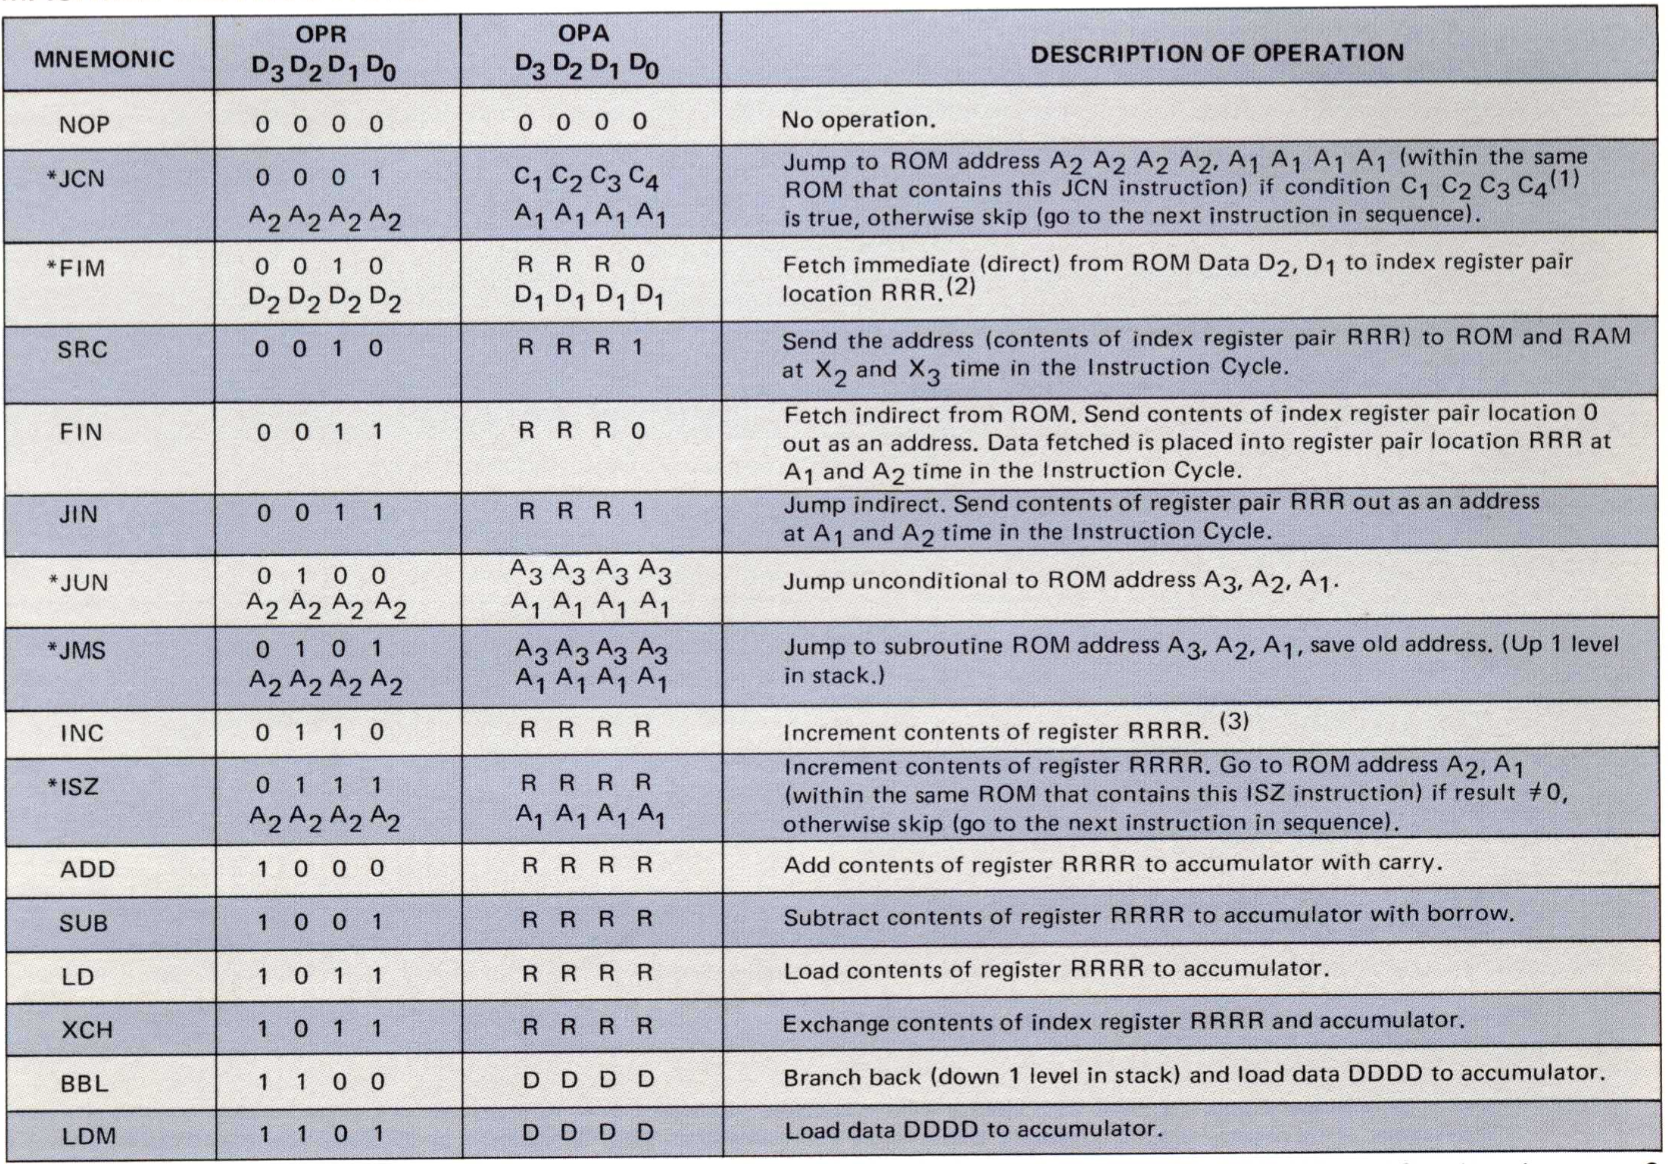
\includegraphics[width=0.8\linewidth]{images/instruction_machine.png}
	\end{figure}
\end{frame}

\begin{frame}
	\frametitle{Intel 4004 Spezifikation}
	\begin{itemize}
		\item Technik: PMOS Transistoren
		\item Strukturbreite: 10$\mu$m
		\item Transistorzahl: 2300
		\item Taktfrequenz: 740 KHz
		\item Dauer eines Befehlszyklus: 10.8 $\mu$s
		\item 92000 Befehle pro Sekunde
		\item Addition 2er 8 stelligen Zahlen: 850 $\mu$s
	\end{itemize}
\end{frame}

\subsection{Auswirkungen auf die Prozessorentwicklung}
\begin{frame}
	\frametitle{Auswirkungen auf die Prozessorentwicklung}
	\begin{itemize}
		\item Intel zögert Rechte von Busicom zurückzukaufen, da Prozessormarkt zu klein
		\item {\grqq}Revolution{\grqq} erst nachdem Intel weitere Developer Tools zur Verfügung stellt
		\item Weiterproduziert bis 1986
		\item Basis für den Intel 8080
		\item Intel hat heute einen Marktanteil von 80$\%$ bei PC-Mikroprozessoren
	\end{itemize}
\end{frame}

\begin{frame}
	\frametitle{Geschichte des MCS-4}
	\framesubtitle{1971 - MCS-4 Werbung}
	\begin{figure}[ht]
		\includegraphics[width=0.9\linewidth]{images/intel_ad.png}
	\end{figure}
\end{frame}


		\chapter{TMS-1000}

\newpage

\section{Geschichte}

W{\"a}hrend Intel es erstmals schaffte alle Bausteine eines Prozessors auf einem Mikrochip zu vereinigen, implementierte Texas Instruments parallel zus{\"a}tzlich Peripherie auf dem Chip und schuf so den ersten Mikrocontroller, welcher auch System-on-a-Chip genannt wurde. \\
Texas Instruments wurde 1951 von Cecil Howard Green, Jon Erik Jonsson, Eugene McDermott und Henry Bates Peacock gegr{\"u}ndet. Das Unternehmen war unter anderem f{\"u}r den ersten integrierten Schaltkreis bekannt. Die Konstruktion eines System-on-a-Chip gelang erstmal den Ingeneuren Gary Boone und Michael Cochran mit dem Controller TMS-1000 im Jahre 1971. Texas Instruments stellte verschiedene Versionen des TMS-1000 her, die in Gr{\"o}{\ss}e des ROM und RAM Speichers variierten. Anfangs verwendete die Firma die Controller nur in eigenen Produkten, vor allem Taschenrechner, wie der SR-16, welcher 1972 auf den Markt kam. Die Firma ist aus diesem Grund und aufgrund der zahlreichen Nachfolger f{\"u}r ihre Taschenrechner bekannt. \\
Erst 3 Jahre nach der Erfindung, also 1974, war der TMS-1000 auf dem freien Markt erh{\"a}ltlich. Dies hatte jedoch zur Folge, dass der Markt durch Intel mit ihren Mikroprozessoren schon zum gro{\ss}en Teil eingenommen war. Trotzdem hatte der Controller aufgrund seines extrem niedrigen Preises, 2\$ pro St{\"u}ck, gro{\ss}en Erfolg auf dem Markt. Der TMS-1000 half dadurch die moderne Elektronik f{\"u}r jedermann zug{\"a}ngig zu machen. Der Controller fand nicht nur in Taschenrechnern Verwendung, sondern auch in ersten Handheld-Ger{\"a}ten, Jukeboxen, T{\"u}rklingeln, Uhren und vielen mehr. Bis zum heutigen Tag wurden ca. 100 Millionen Controller verkauft.

\section{Mikrocontroller}
\subsection{Aufbau}
Mikrocontroller werden nicht zu Unrecht System-on-a-chip genannt und der Aufbau eines Controllers kann daher sehr gut mit den Bestandsteilen eines Computers verglichen werden. Im folgenden werden die Komponenten eines Computers und die Bestandteile eines Mikrocontrollers verglichen. Au{\ss}erdem wird die Aufgabe der einzelnen Bauteile des Controllers beschrieben. 

\newpage
\begin{tabular}{| l | l | l |}
	PC & Mikrocontroller & Aufgabe \\ \hline
	Prozessor & CPU & Der Prozessor f{\"u}hrt die arithmetischen und \\
	 & & logischen Operationen aus \\ \hline
	Arbeitsspeicher & RAM & RAM ist ein tempor{\"a}rer Speicher f{\"u}r Variablen. \\
	& & Verliert den Speicherinhalt nach dem Entfernen \\
	& & der Betriebsspannung \\ \hline
	Festspeicher & ROM & Enth{\"a}lt das Programm \\ \hline
	Takt & Takt & Gibt die Geschwindigkeit der Befehls- \\
	& & folge an \\ \hline
	Peripherie & I/O-Ports & Der Controller enth{\"a}lt einfache Ein- \\
	& & und Ausg{\"a}nge f{\"u}r beispielsweise \\
	& & LEDs, Displays und Schalter \\ \hline
	
\end{tabular}

\subsection{Abgrenzung zu Mikroprozessoren}

Oftmals ist es schwierig eine klare Grenze zwischen Mikroprozessoren und Mikrocontrollern zu ziehen. Das liegt vor allem daran, dass nach einiger Zeit meist Mikrocontroller-Varianten von neuen Mikroprozessor-Architekturen erschienen sind. Die haupst{\"a}chliche Abgrenzung erfolgt durch die Austattung der Zusatzmodule des Chips. W{\"a}hrend ein Mikrocontroller einen Prozessor inklusive Bausteinen wie Speicher, In- und Outputs, Timer, usw. vereint, konzentriert sich ein Mikroprozessor auf seine eigentliche Hauptaufgabe, die Rechengeschwindigkeit. Durch den gesparten Platz auf dem Chip wird diese wesentlich erh{\"o}ht.

\subsection{Architekturen}

Viele der verbauten Mikrocontrollern verwenden 8-Bit-Prozessoren, deren Architektur auf die 1970er Jahre zur{\"u}ckzuf{\"u}hren ist. Allerdings gibt es auch 4-, 16- und 32-Bit Mikrocontroller. Die ersten Controller die gebaut wurden waren dabei 4-Bit-Controller und sind deswegen heutzutage noch stark vertreten. Den gr{\"o}{\ss}ten Marktanteil haben mittlerweile die 32-Bit-Controller da die meisten heutigen Mikrocontroller auf Prozessorkernen basieren, von denen 8- und 16-Bit Prozessoren fast nicht mehr hergestellt werden.

\section{TMS-1000}

\subsection{Allgemeine Daten}

Der TMS-1000 geh{\"o}rt zur Familie der 4-Bit Mikrocontroller. Die Gr{\"o}{\ss}e des ROMs des Controllers betr{\"a}gt 8.192 Bit, w{\"a}hrend die des RAMs 256 Bit betr{\"a}gt. Die maximale Spannung, welche an der Clock und sowohl an den Eingang- und Ausgang-Pins angelegt werden darf, bemisst sich auf 20 Volt. Durch die intern verbauten Oszilliatoren kann der Controller einen Takt von bis zu 0,4 MHz erreichen. Jede Instruktion ben{\"o}tigt 6 Oszilliatoren-Zyklen um vollst{\"a}ndig ausgef{\"u}hrt zu werden. Insgesamt verf{\"u}gt der TMS-1000 {\"u}ber 43 Basisinstruktionen, 12 fixierte und 31 programmierbare. 

\subsection{Pins}

Der TMS-1000 verf{\"u}gt {\"u}ber insgesamt 28 Pins. 

\begin{figure}[!htb]
	\centering
		\includegraphics[width=0.40\textwidth]{figures/pins_TMS1000.PNG}
	\caption{Skizze der Pins}
	\label{fig:pins_TMS1000}
\end{figure}

\newpage

\begin{tabular}{| l | l | l |}
Bezeichnung & Anzahl & Aufgabe \\ \hline
R-Output & 11 & F{\"u}r die Ausgabe von Kontroll-Daten zust{\"a}ndig \\ \hline
O-Output & 8 & Gibt den Inhalt des Akkumulators und das Status-Logic-Bit aus \\ \hline
Oszillatoren & 2 & Zust{\"a}ndig f{\"u}r den Takt des Controllers \\ \hline
Power-Supply & 2 & Versorgt den Controller mit Spannung \\ \hline
K-Input & 4 & Eingang f{\"u}r 4-Bit zur Verwendung im Programm \\ \hline
INIT & 1 & Initialisiert oder setzt die Hardware zur{\"u}k \\ \hline
\end{tabular}

\subsection{Aufbau \& Funktionsweise}

Der folgende Abschnitt befasst sich mit dem Aufbau und der Funktionsweise der Hardware des Mikrocontrollers TMS-1000. 

\begin{figure}[!htb]
	\centering
		\includegraphics[width=0.75\textwidth]{figures/schaltbild.PNG}
	\caption{Schaltbild des TMS-1000}
	\label{fig:schaltbild}
\end{figure}

\subsubsection{ROM - Read Only Memory}

Der Festspeicher besteht aus 16 Seiten, welche je 64 W{\"o}rter enthalten. Jedes Wort ist dabei 8 Bit gro{\ss}. Es werden 4 verschiedene Register benutzt um den Speicher zu adressieren. \\
\\
Das Page Adress Register(PA): Dieses Register enth{\"a}lt die aktuelle Seitenzahl, an dem sich das Programm zur Zeit befindet. Das Register ist 4-Bit gro{\ss}, um alle Seiten von 0 bis 15 adressieren zu k{\"o}nnen. \\
Das Page Buffer Register(PB): Das PB-Register wird mit einer neuen Seitenadresse geladen und nach einer erfolgreichen Branch oder Subroutinen-Operation wird die Adresse in das PA-Register geladen. Aus diesem Grund entspricht die Gr{\"o}{\ss}e des Registers der des PA-Registers \\
Das Program Counter Register(PC): Dieses Register enth{\"a}lt das aktuelle Wort der Seite, in dem sich das Programm zur Zeit befindet. Um alle 64 W{\"o}rter adressieren zu k{\"o}nnen enth{\"a}lt das Register 6 Bit. \\
Das Subroutine Return Register(SR): In dem SR-Register wird bei einer Call Operation das aktuelle Wort des Porgramms gespeichert, um bei einer Return Instruktion zum urspr{\"u}nglichen Wort zur{\"u}ckkehren zu k{\"o}nnen. 

\subsubsection{Branching \& Subroutinen}

Branching und Subroutinen sind ein essenzieller Teil der im Ablauf eines Mikrocontroller-Programms. Ein Branch ist mit einer herk{\"o}mmlichen if-Abfrage aus einer beliebigen Programmiersprache gleichzusetzen. Der Branch wird erfolgreich ausgef{\"u}hrt, wenn das Status-Logic-Bit gesetzt ist. Das Bit ist zwar standardm{\"a}{\ss}ig gleich 1, kann durch Rechenoperationen oder Vergleiche durch die Recheneinheit gleich 0 gesetzt werden. Nach einem Instruktionszyklus wird der Zustand wieder zur{\"u}ckgesetzt. Bei erfolgreicher Ausf{\"u}hrung eines Branches wird das PB-Register in das PA-Register geladen. \\
\\
Subroutinen sind sehr {\"a}hnlich zu Branch Instruktionen. Bei einer erfolgreichen Call-Instruktion springt das Programm an eine andere Adresse im ROM. Bei einer Return-Instruktion kehrt das Programm zu dem urpr{\"u}nglichen Call-Statement zur{\"u}ck. Die Subroutine wird genau wie bei einem Branch nur ausgef{\"u}hrt, wenn das Status-Logic-Bit gesetzt ist. Zus{\"a}tzlich muss jedoch das so genannte Call-Latch gesetzt sein. In diesem Fall wird der Inhalt des PA-Registers mit dem des PB-Registers vertauscht. Die Adresse des PC-Registers wird in dem SR-Register zwischengespeichert. Bei der Return Instruktion werden die tempor{\"a}r gespeicherten Adressen wieder in das PA- und PC-Register geladen. Es ist nicht m{\"o}glich eine Call Instruktion innerhalb einer Call Instruktion aufzurufen, ohne dass die korrekte Return-Adresse verloren geht.

\subsubsection{RAM - Random Access Memory}

Der RAM-Speicher besteht aus 4 Dateien, welche jede 16 W{\"o}rter enthalten. Jedes Wort ist dabei 4 Bit gro{\ss}. Der Speicher wird durch 2 Register X und Y adressiert. Das X-Register gibt dabei die Datei an, das Y-Register das Wort.\\
Der Input erfolgt durch den Write-Multiplexer. Sowohl das Akkumulator Register als auch die Constant and K Input Logic (CKI) k{\"o}nnen in den Speicher schreiben. Der Read-Bus {\"u}bernimmt den Output des RAMs. Der Bus schreibt das Wort entweder in den P-Multiplexer oder den N-Multiplexer, welche beide in die Recheneinheit f{\"u}hren. Die Recheneinheit leitet die Daten entweder in das Y oder Akkumulator Register. \\
Dem Programmierer des Controllers steht es frei, wie er sich den Speicher einteilt. Typischerweise werden die ersten 7 W{\"o}rter jeder Seite f{\"u}r als Register verwendet. Der Rest wird durch beispielsweise Pointer, Event Counter oder Flags bef{\"u}llt. Diese sollten sich wenn m{\"o}glich in der gleichen Datei gespeichert sein, in der auch die Register liegen mit dem sie interagieren.

\subsubsection{Constant \& K Input Logic}

Die CKI Logik selektiert entweder die 4 K-Input Bit oder eine 4-Bit Konstante aus dem ROM und legt diese auf den CKI Daten Bus. Die Konstanten, welche aus dem ROM geliefert werden, werden f{\"u}r Befehle verwendet, welche Konstanten in ihrem Opcode enthalten. Zum Beispiel die Instruktion A8AAC. Diese Instruktion addiert die Zahl 8 zu dem Inhalt des Akkumulators und speichert das Ergebnis wiederum im Akkumulator. Der CKI Daten Bus kann die das 4-Bit Wort entweder in einen der beiden Adder leiten, die zur Recheneinheit f{\"u}hren, oder {\"u}ber den Write-Multiplexer in den RAM-Speicher.

\subsubsection{Y-Register}

Das Y-Register adressiert zusammen mit dem X-Register den RAM-Speicher. Au{\ss}erdem adressiert das Register das R-Output Register, welches die individuellen Latches setzt und resettet. Das Y-Register wird zus{\"a}tzlich als Arbeitsregister bezeichnet, da tempor{\"a}r ROM W{\"o}rter gespeichert werden k{\"o}nnen und sich das Register sehr gut als Counter eignet.

\subsubsection{R- und O-Output}

Der TMS-1000 hat zwei verschiede Arten an Output, R und O. Die R-Outputs werden f{\"u}r Kontroll Daten verwendet. Diese Kontroll Daten werden f{\"u}r externe Ger{\"a}te verwendet oder Status-Logic-Outputs, wie zum Beispiel Overflow. \\
Das O-Output Register enth{\"a}lt den Inhalt des Akkumulators, sowie das Status-Logic-Bit. Durch ein PLA\footnote{Programmable Logic Array} werden die 5 Bit zu den 8 Output-Bit kodiert. Der Programmierer kann dabei selbst bestimmen wie er die Ein- und Ausg{\"a}nge verbindet. Das O-Output Register wird generell f{\"u}r die Ausgabe von Daten benutzt im Gegensatz zum R-Output Register.

\subsubsection{Akkumulator \& ALU - Aritmethic Logic Unit}

Das Akkumulator Register ist sehr wichtig, da es mit der ALU dem RAM-Speicher und dem O-Output Register interagiert. Haupts{\"a}chlich wird das Register f{\"u}r Additionen und Substraktionen verwendet. Au{\ss}erdem werden im Akkumulator Konstanten zwischengespeichert und alle Variablendaten, die in den RAM-Speicher geschrieben werden sollen, m{\"u}ssen den Akkumulator durchlaufen. \\
Die ALU ist ein 4-Bit Adder und Komparator. Er kann addieren, subtrahieren und logische Vergleiche durchf{\"u}hren. Seine Inputs bekommt die Einheit durch 2 4-Bit Multiplexer, die ihren Inhalt durch das Y-Register, die CKI, den RAM-Speicher oder den Akkumulator bekommen. Das Ergebnis wird je nach Instruktion entweder im Y-Register oder Akkumulator gespeichert. Die Substraktion wird durch die two's complement arithmetic ausgef{\"u}hrt. Bei dieser Arithmetik wird der Subtrahend invertiert und auf den Minuend addiert. \\
Die ALU setzt au{\ss}erdem das Status-Logic-Bit. Das Bit kann nicht nur bei logischen Vergleichen gesetzt werden, sonder kann auch bei arithmetischen Operationen als Carry gesetzt werden f{\"u}r beispielsweise {\"U}bertr{\"a}ge.
\newpage

\begin{figure}[!htb]
	\centering
		\includegraphics[width=0.75\textwidth]{figures/ALU_TMS1000.PNG}
	\caption{Eine Skizze der arithmetisch logischen Einheit}
	\label{fig:ALU_TMS1000}
\end{figure}

\subsubsection{Instruction-Decoders}

Der TMS-1000 enth{\"a}lt zwei logische Bl{\"o}cke, die jeweils die 8-Bit Instruktionen in die verschiedenen Mikroinstruktionen dekodiert. Der erste Dekodierer, der "`Fixed instruction decoder"', kann nicht modifiziert werden und aktiviert 12 fixierte Mikroinstruktionen. \\
Die restlichen 31 Basis Instruktionen sind die programmierbaren Instruktionen. Diese werden durch den zweiten Dekodierer, den "`Programmable instruction PLA"', definiert. Standardm{\"a}{\ss}ig sind diese f{\"u}r den Programmierer vordefiniert. Sie k{\"o}nnen aber auch durch das umprogrammieren des PLAs umdefiniert werden. Dabei stehen dem Dekodierer 16 Mikroinstruktionen zur Verf{\"u}gung, die beliebig kombiniert werden k{\"o}nnen.

\newpage
\subsection{Befehlssatz}

\subsubsection{Befehlsformate}

Die 43 Basisinstruktionen werden durch jewils eine der 4 Instruktionsformate beschrieben. Jedes Format enth{\"a}lt dabei 8-Bit, welche wie folgt aufgeteilt sind:

\begin{figure}[!htb]
	\centering
		\includegraphics[width=0.5\textwidth]{figures/I1.PNG}
	\caption{Instruktionsformat 1}
	\label{fig:I1}
\end{figure}

Das erste Format besteht aus 2 Bit Op-Code und einem 6-Bit ROM-Wort. Dieses Format wird f{\"u}r Branch und Subroutinen-Control benutzt. Das ROM-Wort beschreibt die zu ladene Adresse.

\begin{figure}[!htb]
	\centering
		\includegraphics[width=0.5\textwidth]{figures/I2.PNG}
	\caption{Instruktionsformat 2}
	\label{fig:I2}
\end{figure}

Das zweite Format besteht aus 4-Bit Op-Code und einer 4-Bit Konstante. Es wird benutzt, um Konstanten in ein Register oder in den RAM-Speicher zu schreiben. Bei diesem Format ist das Most-significant-Bit und das Least-significant-Bit vertauscht.

\begin{figure}[!htb]
	\centering
		\includegraphics[width=0.5\textwidth]{figures/I3.PNG}
	\caption{Instruktionsformat 3}
	\label{fig:I3}
\end{figure}

Das dritte Format besteht aus 6-Bit Op-Code und einem 2-Bit gro{\ss}en Operanden. Der Operand adresiert ein bestimmtes Bit aus einem RAM-Wort, welches wiederum durch das X und Y Register adressiert wird.

\begin{figure}[!htb]
	\centering
		\includegraphics[width=0.5\textwidth]{figures/I4.PNG}
	\caption{Instruktionsformat 4}
	\label{fig:I4}
\end{figure}

Das vierte und letzte Format besteht ausschlie{\ss}lich aus Op-Code. Dieses Format wird f{\"u}r Instruktionen benutzt, die immer dasselbe erledigen und deswegen keine Konstanten ben{\"o}tigen.

\subsubsection{Instruktionsbeispiele}

Das erste Beispiel ist eine arithmetische Instruktion, AMAAC. Die Instruktion addiert ein Wort aus dem RAM-Speicher auf den Inhalt des Akkumulators. Das Ergebnis wird im Akkumulator gespeichert. Die Instruktion aktiviert 4 der programmierbaren Mikroinstruktionen. MTP l{\"a}dt ein Wort aus dem Speicher in den P-Multiplexer, ATN den Akkumulator in den N-Multipelexer. C8 setz das Status-Logic-Bit bei einem {\"U}bertrag. AUTA l{\"a}sst das Ergebnis der Addition im Akkumulator speichern. \\
\\
Das zweite Beispiel, ALEC, ist ein arithmetischer Vergleich. Die Instruktion, welche durch das zweite Format beschrieben wird, vergleicht den Inhalt des Akkumulators mit einer Konstante, die mit der Instruktion {\"u}bergeben wird. Wenn der Akkumulator kleiner oder gleich gro{\ss} wie die Konstante ist, wird das Status-Logic-Bit gesetzt. Auch bei dieser Instruktion, werden 4 der programmierbaren Mikroinstruktionen aktiviert. CKP l{\"a}dt die Konstante in den P-Multiplexer, NATN den invertierten Inhalt des Akkumulators in den N-Multiplexer, da der Vergleich {\"u}ber eine Subtraktion erfolgt. CIN addiert 1 auf die Summe, um die Subtraktion zu vervollst{\"a}ndigen. C8 setzt erneut das Status-Logic-Bit bei einem {\"U}bertrag. 

\section{Verwendung Mikrocontroller}

Mikrocontroller spielen eine wichtige Rolle in vielen elektronischen Ger{\"a}ten. Sie finden Verwendung in eingebetteten Systemen und sind im Alltag oft unbemerkt. In Leistung und Austattung sind sie meist auf eine Anwendung angepasst, um maximale Effizienz gew{\"a}hrleisten zu k{\"o}nnen.  \\
Mikrocontroller werden nicht nur in der Unterhaltungselektronik wie CD- und DVD-Spielen verwendet, sondern auch f{\"u}r Gebrauchsgegenst{\"a}nde wie Waschmaschinen oder K{\"u}hlschr{\"a}nke. Die hohe Verwendung der Mikrocontroller l{\"a}sst sich zum einen auf die extrem billigen Preise zur{\"u}ckf{\"u}hren, zum anderen auf die extrem hohe Zuverl{\"a}ssigkeit. Laut Texas Instruments f{\"a}llt ein TMS-1000 im Durchschnitt nur ein einziges mal innerhalb von 240 Jahren aus. \\
Der TMS-1000 ist vor allem f{\"u}r seine Verwendung in den von Texas Instruments produzierten Taschenrechnern bekannt. Jedoch wurde der Controller auch unter anderem in T{\"u}rklingeln und diversen Spielen verwendet. Dazu geh{\"o}rt zum Beispiel das elektronische Hand-Held "`Speak \& Spell"', welches 1978 von Texas Instruments auf den Markt gebracht wurde. 

\begin{figure}[!htb]
	\centering
		\includegraphics[width=0.4\textwidth]{figures/sp_sp.JPG}
	\caption{Das Hand-Held Speak \& Spell}
	\label{fig:sp_sp}
\end{figure}
	\newpage
\section{Schluss}
Test Schluss
\end{spacing}
\newpage
\thispagestyle{empty}
\null


%\input{appendices}
	
% Generierung des Literaturverzeichnisses
%\bibliography{/path/to/your/.bib/file}

\end{document}
